\documentclass[]{book}
\usepackage{lmodern}
\usepackage{amssymb,amsmath}
\usepackage{ifxetex,ifluatex}
\usepackage{fixltx2e} % provides \textsubscript
\ifnum 0\ifxetex 1\fi\ifluatex 1\fi=0 % if pdftex
  \usepackage[T1]{fontenc}
  \usepackage[utf8]{inputenc}
\else % if luatex or xelatex
  \ifxetex
    \usepackage{mathspec}
  \else
    \usepackage{fontspec}
  \fi
  \defaultfontfeatures{Ligatures=TeX,Scale=MatchLowercase}
\fi
% use upquote if available, for straight quotes in verbatim environments
\IfFileExists{upquote.sty}{\usepackage{upquote}}{}
% use microtype if available
\IfFileExists{microtype.sty}{%
\usepackage{microtype}
\UseMicrotypeSet[protrusion]{basicmath} % disable protrusion for tt fonts
}{}
\usepackage[margin=1in]{geometry}
\usepackage{hyperref}
\PassOptionsToPackage{usenames,dvipsnames}{color} % color is loaded by hyperref
\hypersetup{unicode=true,
            pdftitle={Intro to Regression Analysis},
            pdfauthor={Maria Tackett},
            colorlinks=true,
            linkcolor=Maroon,
            citecolor=Blue,
            urlcolor=Blue,
            breaklinks=true}
\urlstyle{same}  % don't use monospace font for urls
\usepackage{natbib}
\bibliographystyle{apalike}
\usepackage{color}
\usepackage{fancyvrb}
\newcommand{\VerbBar}{|}
\newcommand{\VERB}{\Verb[commandchars=\\\{\}]}
\DefineVerbatimEnvironment{Highlighting}{Verbatim}{commandchars=\\\{\}}
% Add ',fontsize=\small' for more characters per line
\usepackage{framed}
\definecolor{shadecolor}{RGB}{248,248,248}
\newenvironment{Shaded}{\begin{snugshade}}{\end{snugshade}}
\newcommand{\KeywordTok}[1]{\textcolor[rgb]{0.13,0.29,0.53}{\textbf{#1}}}
\newcommand{\DataTypeTok}[1]{\textcolor[rgb]{0.13,0.29,0.53}{#1}}
\newcommand{\DecValTok}[1]{\textcolor[rgb]{0.00,0.00,0.81}{#1}}
\newcommand{\BaseNTok}[1]{\textcolor[rgb]{0.00,0.00,0.81}{#1}}
\newcommand{\FloatTok}[1]{\textcolor[rgb]{0.00,0.00,0.81}{#1}}
\newcommand{\ConstantTok}[1]{\textcolor[rgb]{0.00,0.00,0.00}{#1}}
\newcommand{\CharTok}[1]{\textcolor[rgb]{0.31,0.60,0.02}{#1}}
\newcommand{\SpecialCharTok}[1]{\textcolor[rgb]{0.00,0.00,0.00}{#1}}
\newcommand{\StringTok}[1]{\textcolor[rgb]{0.31,0.60,0.02}{#1}}
\newcommand{\VerbatimStringTok}[1]{\textcolor[rgb]{0.31,0.60,0.02}{#1}}
\newcommand{\SpecialStringTok}[1]{\textcolor[rgb]{0.31,0.60,0.02}{#1}}
\newcommand{\ImportTok}[1]{#1}
\newcommand{\CommentTok}[1]{\textcolor[rgb]{0.56,0.35,0.01}{\textit{#1}}}
\newcommand{\DocumentationTok}[1]{\textcolor[rgb]{0.56,0.35,0.01}{\textbf{\textit{#1}}}}
\newcommand{\AnnotationTok}[1]{\textcolor[rgb]{0.56,0.35,0.01}{\textbf{\textit{#1}}}}
\newcommand{\CommentVarTok}[1]{\textcolor[rgb]{0.56,0.35,0.01}{\textbf{\textit{#1}}}}
\newcommand{\OtherTok}[1]{\textcolor[rgb]{0.56,0.35,0.01}{#1}}
\newcommand{\FunctionTok}[1]{\textcolor[rgb]{0.00,0.00,0.00}{#1}}
\newcommand{\VariableTok}[1]{\textcolor[rgb]{0.00,0.00,0.00}{#1}}
\newcommand{\ControlFlowTok}[1]{\textcolor[rgb]{0.13,0.29,0.53}{\textbf{#1}}}
\newcommand{\OperatorTok}[1]{\textcolor[rgb]{0.81,0.36,0.00}{\textbf{#1}}}
\newcommand{\BuiltInTok}[1]{#1}
\newcommand{\ExtensionTok}[1]{#1}
\newcommand{\PreprocessorTok}[1]{\textcolor[rgb]{0.56,0.35,0.01}{\textit{#1}}}
\newcommand{\AttributeTok}[1]{\textcolor[rgb]{0.77,0.63,0.00}{#1}}
\newcommand{\RegionMarkerTok}[1]{#1}
\newcommand{\InformationTok}[1]{\textcolor[rgb]{0.56,0.35,0.01}{\textbf{\textit{#1}}}}
\newcommand{\WarningTok}[1]{\textcolor[rgb]{0.56,0.35,0.01}{\textbf{\textit{#1}}}}
\newcommand{\AlertTok}[1]{\textcolor[rgb]{0.94,0.16,0.16}{#1}}
\newcommand{\ErrorTok}[1]{\textcolor[rgb]{0.64,0.00,0.00}{\textbf{#1}}}
\newcommand{\NormalTok}[1]{#1}
\usepackage{longtable,booktabs}
\usepackage{graphicx,grffile}
\makeatletter
\def\maxwidth{\ifdim\Gin@nat@width>\linewidth\linewidth\else\Gin@nat@width\fi}
\def\maxheight{\ifdim\Gin@nat@height>\textheight\textheight\else\Gin@nat@height\fi}
\makeatother
% Scale images if necessary, so that they will not overflow the page
% margins by default, and it is still possible to overwrite the defaults
% using explicit options in \includegraphics[width, height, ...]{}
\setkeys{Gin}{width=\maxwidth,height=\maxheight,keepaspectratio}
\IfFileExists{parskip.sty}{%
\usepackage{parskip}
}{% else
\setlength{\parindent}{0pt}
\setlength{\parskip}{6pt plus 2pt minus 1pt}
}
\setlength{\emergencystretch}{3em}  % prevent overfull lines
\providecommand{\tightlist}{%
  \setlength{\itemsep}{0pt}\setlength{\parskip}{0pt}}
\setcounter{secnumdepth}{5}
% Redefines (sub)paragraphs to behave more like sections
\ifx\paragraph\undefined\else
\let\oldparagraph\paragraph
\renewcommand{\paragraph}[1]{\oldparagraph{#1}\mbox{}}
\fi
\ifx\subparagraph\undefined\else
\let\oldsubparagraph\subparagraph
\renewcommand{\subparagraph}[1]{\oldsubparagraph{#1}\mbox{}}
\fi

%%% Use protect on footnotes to avoid problems with footnotes in titles
\let\rmarkdownfootnote\footnote%
\def\footnote{\protect\rmarkdownfootnote}

%%% Change title format to be more compact
\usepackage{titling}

% Create subtitle command for use in maketitle
\providecommand{\subtitle}[1]{
  \posttitle{
    \begin{center}\large#1\end{center}
    }
}

\setlength{\droptitle}{-2em}

  \title{Intro to Regression Analysis}
    \pretitle{\vspace{\droptitle}\centering\huge}
  \posttitle{\par}
    \author{Maria Tackett}
    \preauthor{\centering\large\emph}
  \postauthor{\par}
      \predate{\centering\large\emph}
  \postdate{\par}
    \date{2019-05-14}

\usepackage{booktabs}

\begin{document}
\maketitle

{
\hypersetup{linkcolor=black}
\setcounter{tocdepth}{1}
\tableofcontents
}
\listoftables
\listoffigures
\chapter{Beginning of the Book}\label{beginning-of-the-book}

This is the introduction to the book.

This work is licensed under the
\href{http://creativecommons.org/licenses/by-nc-sa/4.0/}{Creative
Commons Attribution-NonCommercial-ShareAlike 4.0 International License}.

\chapter{Introduction}\label{intro}

You can label chapter and section titles using \texttt{\{\#label\}}
after them, e.g., we can reference Chapter \ref{intro}. If you do not
manually label them, there will be automatic labels anyway, e.g.,
Chapter \ref{methods}.

Figures and tables with captions will be placed in \texttt{figure} and
\texttt{table} environments, respectively.

\begin{Shaded}
\begin{Highlighting}[]
\KeywordTok{par}\NormalTok{(}\DataTypeTok{mar =} \KeywordTok{c}\NormalTok{(}\DecValTok{4}\NormalTok{, }\DecValTok{4}\NormalTok{, .}\DecValTok{1}\NormalTok{, .}\DecValTok{1}\NormalTok{))}
\KeywordTok{plot}\NormalTok{(pressure, }\DataTypeTok{type =} \StringTok{'b'}\NormalTok{, }\DataTypeTok{pch =} \DecValTok{19}\NormalTok{)}
\end{Highlighting}
\end{Shaded}

\begin{figure}

{\centering 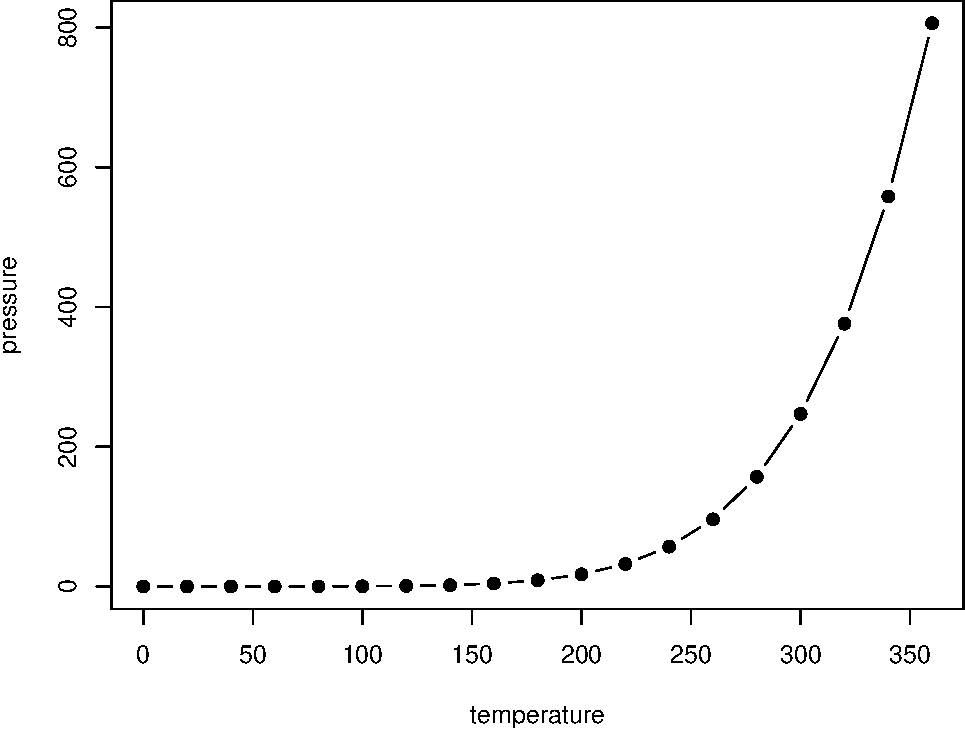
\includegraphics[width=0.8\linewidth]{introregression_files/figure-latex/nice-fig-1} 

}

\caption{Here is a nice figure!}\label{fig:nice-fig}
\end{figure}

Reference a figure by its code chunk label with the \texttt{fig:}
prefix, e.g., see Figure \ref{fig:nice-fig}. Similarly, you can
reference tables generated from \texttt{knitr::kable()}, e.g., see Table
\ref{tab:nice-tab}.

\begin{Shaded}
\begin{Highlighting}[]
\NormalTok{knitr}\OperatorTok{::}\KeywordTok{kable}\NormalTok{(}
  \KeywordTok{head}\NormalTok{(iris, }\DecValTok{20}\NormalTok{), }\DataTypeTok{caption =} \StringTok{'Here is a nice table!'}\NormalTok{,}
  \DataTypeTok{booktabs =} \OtherTok{TRUE}
\NormalTok{)}
\end{Highlighting}
\end{Shaded}

\begin{table}[t]

\caption{\label{tab:nice-tab}Here is a nice table!}
\centering
\begin{tabular}{rrrrl}
\toprule
Sepal.Length & Sepal.Width & Petal.Length & Petal.Width & Species\\
\midrule
5.1 & 3.5 & 1.4 & 0.2 & setosa\\
4.9 & 3.0 & 1.4 & 0.2 & setosa\\
4.7 & 3.2 & 1.3 & 0.2 & setosa\\
4.6 & 3.1 & 1.5 & 0.2 & setosa\\
5.0 & 3.6 & 1.4 & 0.2 & setosa\\
\addlinespace
5.4 & 3.9 & 1.7 & 0.4 & setosa\\
4.6 & 3.4 & 1.4 & 0.3 & setosa\\
5.0 & 3.4 & 1.5 & 0.2 & setosa\\
4.4 & 2.9 & 1.4 & 0.2 & setosa\\
4.9 & 3.1 & 1.5 & 0.1 & setosa\\
\addlinespace
5.4 & 3.7 & 1.5 & 0.2 & setosa\\
4.8 & 3.4 & 1.6 & 0.2 & setosa\\
4.8 & 3.0 & 1.4 & 0.1 & setosa\\
4.3 & 3.0 & 1.1 & 0.1 & setosa\\
5.8 & 4.0 & 1.2 & 0.2 & setosa\\
\addlinespace
5.7 & 4.4 & 1.5 & 0.4 & setosa\\
5.4 & 3.9 & 1.3 & 0.4 & setosa\\
5.1 & 3.5 & 1.4 & 0.3 & setosa\\
5.7 & 3.8 & 1.7 & 0.3 & setosa\\
5.1 & 3.8 & 1.5 & 0.3 & setosa\\
\bottomrule
\end{tabular}
\end{table}

You can write citations, too. For example, we are using the
\textbf{bookdown} package \citep{R-bookdown} in this sample book, which
was built on top of R Markdown and \textbf{knitr} \citep{xie2015}.

\chapter{Getting Started}\label{getstarted}

This is a chapter about getting started using R and GitHub.

\chapter{Simple Linear Regression}\label{slr}

\part*{Computing Exercises}\label{part-computing-exercises}
\addcontentsline{toc}{part}{Computing Exercises}

\section{Computing: College
Admissions}\label{computing-college-admissions}

The primary goal of today's lab is to give you practice with some of the
tools you will need to conduct regression analysis using R. An
additional goal for today is for you to be introduced to your teams and
practice collaborating using GitHub and RStudio.

\subsection{Packages}\label{packages}

We will use the following packages in today's lab.

\part*{In-Class Exercises}\label{part-in-class-exercises}
\addcontentsline{toc}{part}{In-Class Exercises}

\section{In-Class Exercise: Advertising
Analysis}\label{in-class-exercise-advertising-analysis}

In this mini analysis, we will work with the \texttt{Advertising} data
used in Chapters 2 and 3 of \emph{Introduction to Statistical Learning}.

\section{Data and packages}\label{data-and-packages}

We start with loading the packages we'll use.

We will analyze the advertising and sales data for 200 markets. The
variables we'll use are

\begin{itemize}
\tightlist
\item
  \texttt{tv}: total spending on TV advertising (in \$thousands)
\item
  \texttt{radio}: total spending on radio advertising (in \$thousands)
\item
  \texttt{newspaper}: total spending on newspaper advertising (in
  \$thousands)
\item
  \texttt{sales}: total sales (in \$millions)
\end{itemize}

\section{Analysis}\label{analysis}

We'll begin the analysis by getting quick view of the data:

Next, we can calculate summary statistics for each of the variables in
the data set.

\begin{enumerate}
\def\labelenumi{\arabic{enumi}.}
\tightlist
\item
  What type of advertising has the smallest median spending?
\item
  What type of advertising has the largest variation in spending?
\item
  Describe the shape of the distribution of \texttt{sales}.
\end{enumerate}

We are most interested in understanding how advertising spending affect
sales. One way to quantify the relationship between the variables is by
calculating the correlation matrix.

\begin{enumerate}
\def\labelenumi{\arabic{enumi}.}
\tightlist
\item
  What is the correlation between \texttt{radio} and \texttt{sales}?
  Interpret this value.
\item
  What type of advertising has the strongest linear relationship with
  \texttt{sales}?
\end{enumerate}

Below are visualizations of \texttt{sales} versus each explanatory
variable.

Since \texttt{tv} appears to have the strongest linear relationship with
\texttt{sales}, let's calculate a simple linear regression model using
these two variables.

\begin{enumerate}
\def\labelenumi{\arabic{enumi}.}
\tightlist
\item
  Write the model equation.
\item
  Interpret the intercept in the context of the problem.
\item
  Interpret the slope in the context of the problem.
\end{enumerate}

\section{In-Class Exercise: Beer Data
Analysis}\label{in-class-exercise-beer-data-analysis}

In this analysis, we will analyze the relationship between the amount of
alcohol (\texttt{PercentAlcohol}) and the caloric content
(\texttt{CaloriesPer12Oz}) in domestic beers. Let
\texttt{PercentAlcohol} be the predictor variable and
\texttt{CaloriesPer12Oz} the response variable.

Due to limited class time, we will not do the exploratory data analysis
in this example. In practice, however, you should always start with the
exploratory data analysis.

\emph{You can add your answers to this R Markdown document}.

**1. Calculate a regression model to describe the relationship between
\texttt{PercentAlcohol} and \texttt{CaloriesPer12Oz}. Display the model
output.*

\textbf{2. Does it make sense to interpret the intercept? Why or why
not?}

There are non-alocoholic beers, so it is possible to have a meaningful
interpretation of the intercept. In our data, however, there are very
few beers with less than 3\% alcoholic content, so it would not be wise
to interpret the intercept. It is not safe to assume the same
relationship between \texttt{PercentAlcohol} and
\texttt{CaloriesPer12Oz} hold for beers with 0\% alcohol; this would be
extrapolation.

\textbf{3. Interpret the 95\% confidence interval for the slope in the
context of the data.}

We are 95\% confident that the interval (26.557, 30.620) contains the
true population slope for \texttt{PercentAlcohol}. This means we are
95\% confident that for every 1\% increase in alcohol content, the
number of calories (per 12 oz) is expected to increase between 26.557
and 30.620 calories.

\textbf{4. Find the critical value, \(t^*\), used to calculate the 95\%
confidence interval. The code below is a guide; uncomment and complete
the lines of code to calculate and display the critical value.}

The critical value used to calculate the 95\% confident interval for the
slope is \_\_\_\_\_\_.

\textbf{5. Interpret the test statistic in the context of the data}

The estimated slope of 28.577 is 27.78 standard errors above the
hypothesized mean of 0, assuming there is no linear relationship between
percent alcohol and calories in domestic beers.

\textbf{6. How was the p-value calculated? Fill in the code below to
calculate the p-value. The code below is a guide; uncomment and complete
the lines of code to calculate and display the p-value.}

The p-value is \_\_\_\_\_\_\_. Given there is no linear relationship
between \texttt{PercentAlcohol} and \texttt{CaloriesPer12Oz}, the
probability of obtaining a test statistic with magnitude
\_\_\_\_\_\_\_\_ or more extreme is \_\_\_\_\_\_\_.

\textbf{7. Fill in the code below to calculate the predicted calories
and corresponding 90\% interval for a single beer with alcohol content
of 4.3\%.}

\textbf{8. Fill in the code below to calculate the predicted calories
and corresponding 90\% interval for the subset of beers with alcohol
content of 4.3\%.}

\chapter{Analysis of Variance}\label{anova}

\part*{Computing
Assignments}\label{part-computing-assignments}
\addcontentsline{toc}{part}{Computing Assignments}

\chapter{Multiple Linear Regression}\label{mlr}

\part*{Computing
Assignments}\label{part-computing-assignments-1}
\addcontentsline{toc}{part}{Computing Assignments}

\part*{In-Class Exericses}\label{part-in-class-exericses}
\addcontentsline{toc}{part}{In-Class Exericses}

\chapter{(PART*) Math Notes}\label{part-math-notes}

\chapter{Model Selection}\label{select}

\part*{Computing
Assignments}\label{part-computing-assignments-2}
\addcontentsline{toc}{part}{Computing Assignments}

\part*{In-Class Exericses}\label{part-in-class-exericses-1}
\addcontentsline{toc}{part}{In-Class Exericses}

\part*{Math Notes}\label{part-math-notes-1}
\addcontentsline{toc}{part}{Math Notes}

\chapter{Logistic Regression}\label{logistic}

\part*{Computing
Assignments}\label{part-computing-assignments-3}
\addcontentsline{toc}{part}{Computing Assignments}

\part*{In-Class Exericse}\label{part-in-class-exericse}
\addcontentsline{toc}{part}{In-Class Exericse}

\chapter{Multinomial Logistic Regression}\label{multinom-logistic}

\part*{Computing
Assignments}\label{part-computing-assignments-4}
\addcontentsline{toc}{part}{Computing Assignments}

\part*{In-Class Exericses}\label{part-in-class-exericses-2}
\addcontentsline{toc}{part}{In-Class Exericses}

\chapter{Special Topics}\label{special}

\part*{Computing
Assignments}\label{part-computing-assignments-5}
\addcontentsline{toc}{part}{Computing Assignments}

\part*{In-Class Exericses}\label{part}
\addcontentsline{toc}{part}{In-Class Exericses}

\chapter{Data Sets}\label{data}

\begin{longtable}[]{@{}llll@{}}
\toprule
Data Set & Description & Chapter & Original Source\tabularnewline
\midrule
\endhead
\texttt{advertising.csv} & test & test & test\tabularnewline
\texttt{airbnb\_basic.csv} & test & test & test\tabularnewline
\texttt{airbnb\_details.csv} & test & test & test\tabularnewline
\texttt{beer.csv} & test & test & test\tabularnewline
\texttt{evals\_mod.csv} & test & test & test\tabularnewline
\texttt{fivethirtyeight-recent-grads.R} & test & test &
test\tabularnewline
\texttt{framingham.csv} & test & test & test\tabularnewline
\texttt{gss2016.csv} & test & test & test\tabularnewline
\texttt{KingCountyHouses.csv} & test & test & test\tabularnewline
\texttt{ncbreweries.csv} & test & test & test\tabularnewline
\texttt{recent-grads.csv} & test & test & test\tabularnewline
\texttt{sesame.csv} & test & test & test\tabularnewline
\texttt{sis.csv} & test & test & test\tabularnewline
\texttt{spotify.csv} & test & test & test\tabularnewline
\texttt{test\_songs.csv} & test & test & test\tabularnewline
\bottomrule
\end{longtable}

\chapter{References}\label{refs}

\bibliography{book.bib,packages.bib}


\end{document}
